\section{Experiments}
\label{sec:Experiments}

\textbf{Experiment Strategy:} Each individual experiment is done for 10 times
and average round number for all proposers is calculated every time. Finally
the average round number for the whole experiment in all 10 experiments is
calculated.

\subsection{Initial sleep time}
In this experiment we modify the initial sleep time. The code used for this experiment
is located at the \textit{src/main} folder. We first run the original code launching the
proposers at the same time: \textit{paxy:start([200,200,200])}. Then we run again the code delaying
some of the proposers: \textit{paxy:start([1000,2000,3000])}.

\begin{figure}[h!]
  \centering
    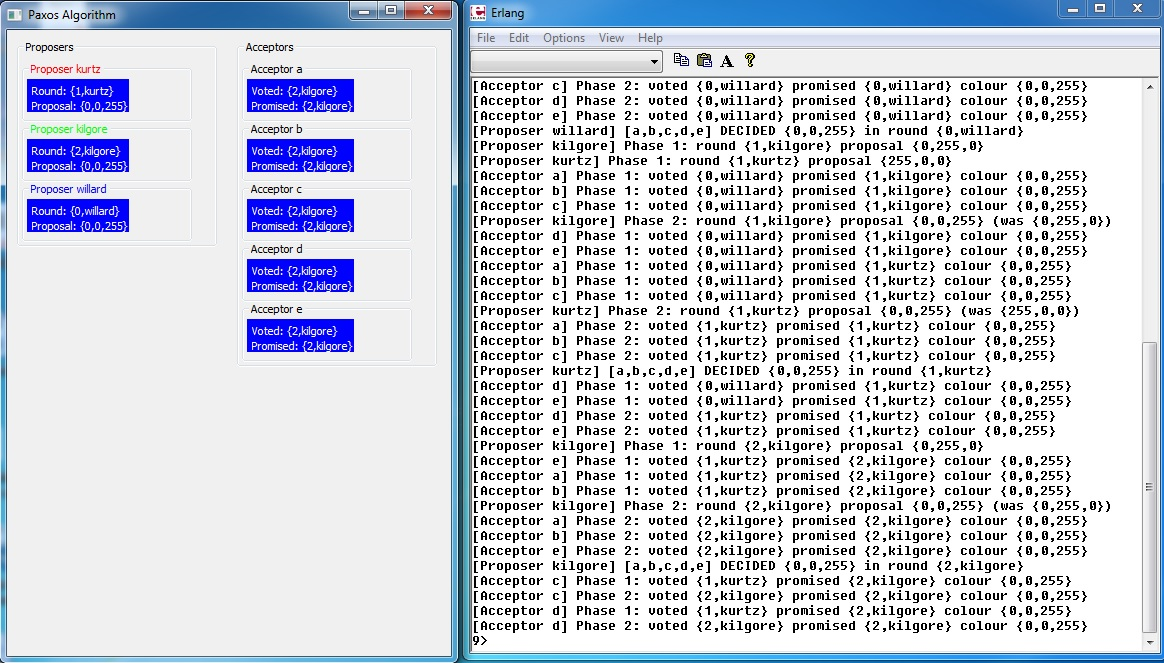
\includegraphics[width=0.95\textwidth]{./3_Experiments/images/initSleep1.jpg}
    \caption{Execution of initial sleep experiment - Default values\label{fig:init_sleep1}}
\end{figure}
\begin{figure}[h!]
  \centering
    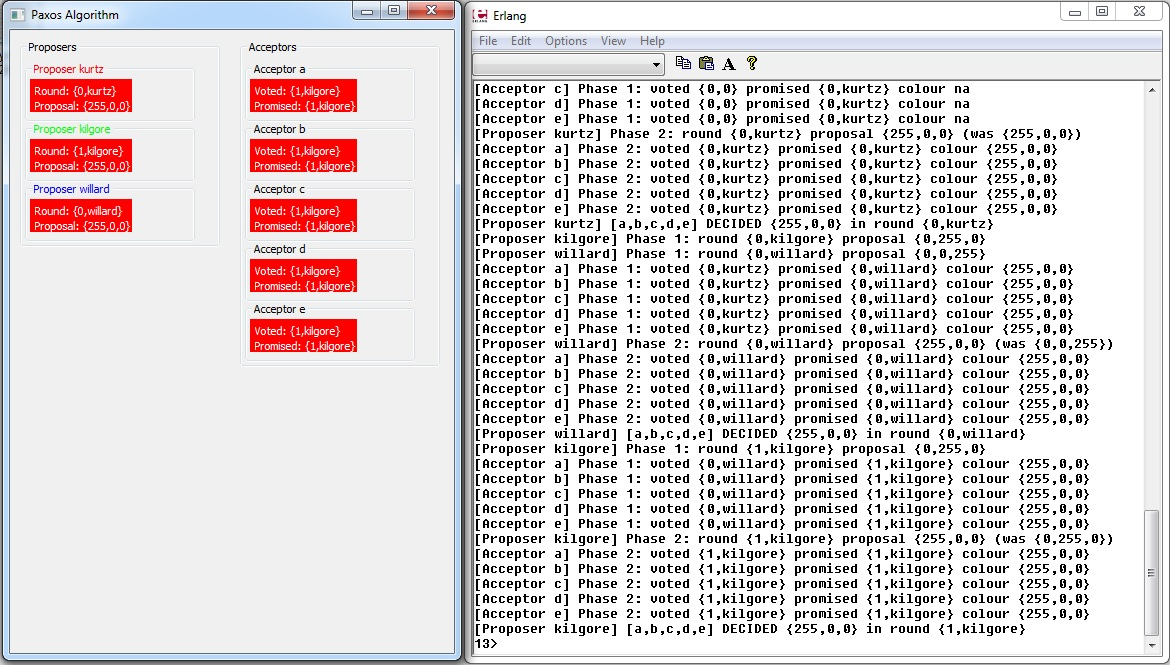
\includegraphics[width=0.95\textwidth]{./3_Experiments/images/initSleep2.jpg}
    \caption{Execution of initial sleep experiment - Incremental values\label{fig:init_sleep2}}
\end{figure}

As shown in Figures \ref{fig:init_sleep1} and \ref{fig:init_sleep2}, wWe find 
that it takes more rounds to reach consensus when proposers run at the 
same time than when they are delayed.
\newpage

\subsection{Introducing Delays in the Acceptor}
In this experiment we delay the prepare messages from the acceptors before sending
them to the proposers and we check if the algorithm terminates or not. For this case
the used code is located under \textit{src/delay} folder.

We do three kinds of experiments with 3 proposers and 5 acceptors:

1. Delays before the prepare messages\newline
\begin{table}[h!]
  \centering
  \begin{tabular}{ |c | c | c | c | c | }
    \hline
                     & Proposer A & Proposer B & Proposer C & Average \\ \hline
    Number of Rounds & 1.1 & 2.6 & 1.9 & 1.87  \\ \hline
  \end{tabular}
  \caption{Results delaying prepare messages}
  \label{table:1}
\end{table}

2. Delays before the accept messages\newline
\begin{table}[h!]
  \centering
  \begin{tabular}{ |c | c | c | c | c | }
    \hline
                     & Proposer A & Proposer B & Proposer C & Average \\ \hline
    Number of Rounds & 1.1 & 3.1 & 2.2 & 2.13  \\ \hline
  \end{tabular}
  \caption{Results delaying accept messages}
  \label{table:2}
\end{table}

3. Delays before the prepare and accept messages\newline
\begin{table}[h!]
  \centering
  \begin{tabular}{ |c | c | c | c | c | }
    \hline
                     & Proposer A & Proposer B & Proposer C & Average \\ \hline
    Number of Rounds & 2 & 2.6 & 2.6 & 2.4  \\ \hline
  \end{tabular}
  \caption{Results delaying prepare messages}
  \label{table:3}
\end{table}
\newpage
\begin{figure}[h!]
  \centering
    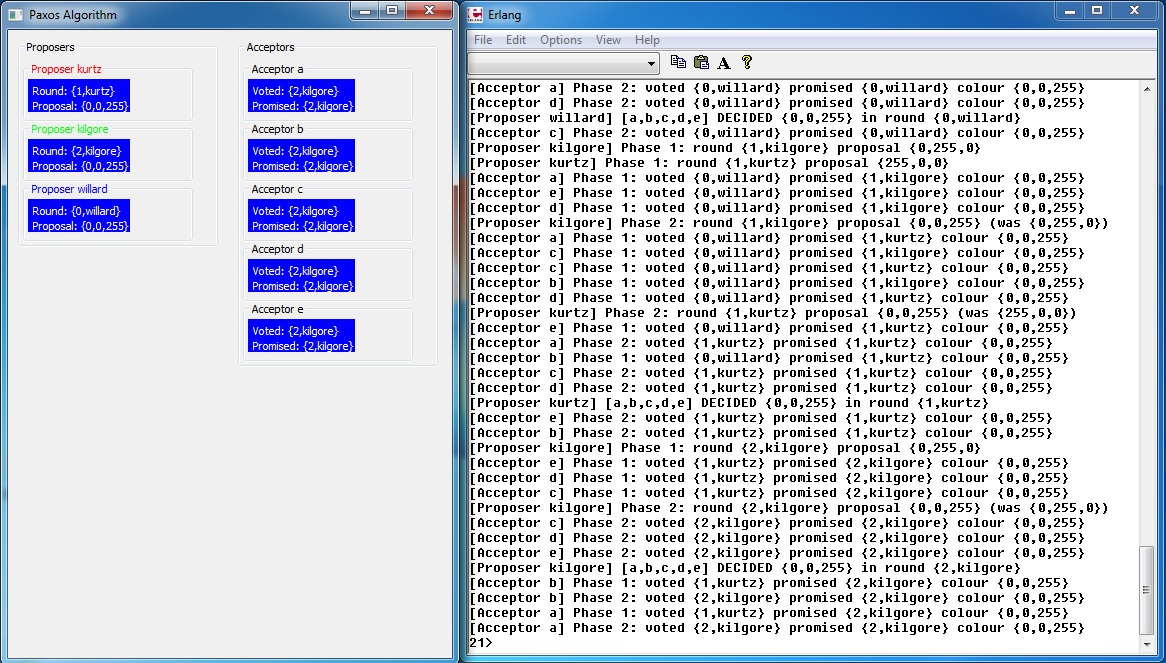
\includegraphics[width=0.95\textwidth]{./3_Experiments/images/delayAll.jpg}
    \caption{Execution with delay on both prepare and accept messages \label{fig:delay_all}}
\end{figure}
As shown in Table \ref{table:1}, Table \ref{table:2} and Table \ref{table:3}, the more delays there are,
the more rounds it takes to reach consensus.


\subsection{Avoid Sending Sorry Messages}
We do three kinds of experiments with 3 proposers and 5 acceptors avoiding to send
sorry messages in different phases: \newline
• Not sending in the 1st phase \newline
• Not sending in the 2nd phase \newline
• Not sending in both phases \newline

\begin{table}[h!]
  \centering
  \begin{tabular}{ |c | c | c | c | c | }
    \hline
                     & Always Send & No send 1 & No send 2 & No send 1-2 \\ \hline
    Number of Rounds & 1 & 1 & 1 & 1  \\ \hline
  \end{tabular}
  \caption{Results avoiding sorry messages}
  \label{table:4}
\end{table}

\begin{figure}[h!]
  \centering
    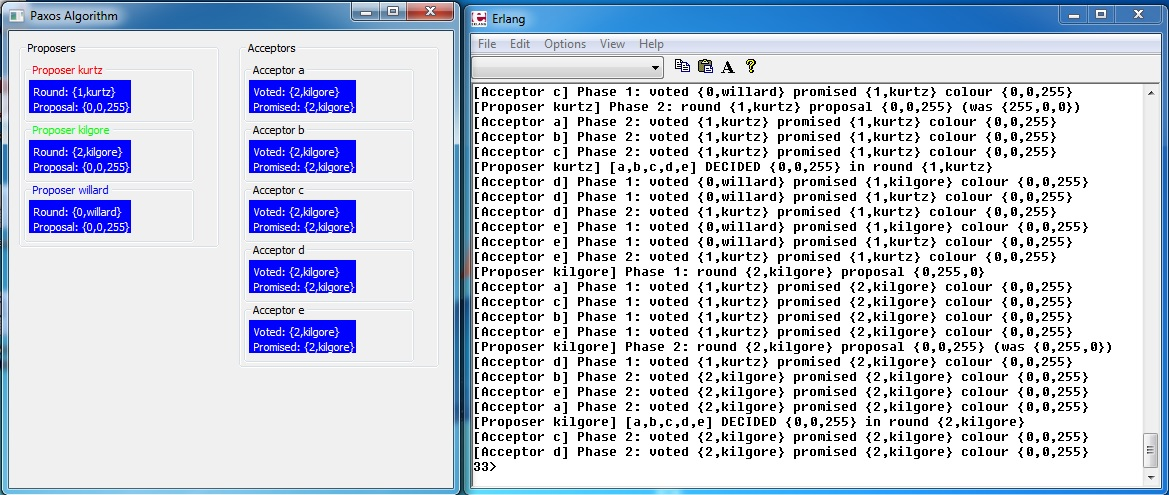
\includegraphics[width=0.95\textwidth]{./3_Experiments/images/nosorry.jpg}
    \caption{Execution avoiding sorry messages \label{fig:nosorry}}
\end{figure}

As we can see in Table \ref{table:4}, not sending sorry messages has no effect
on the number of rounds to reach consensus. Moreover, \textit{Proposers} always
reach consensus even if the sorry messages are avoided or not. 

\subsection{Randomly Dropping Messages in the Acceptor}
In this section we try to evaluate the impact of dropping messages from the 
acceptor. For this purpose the code located under the \textit{src/drop} folder is
used. A first set of experiments is done to check if dropping promise or vote
messages have a different impact on the execution: \newline
– Experiment 1: Only drop 1/10 promise messages\newline
\begin{figure}[h!]
  \centering
    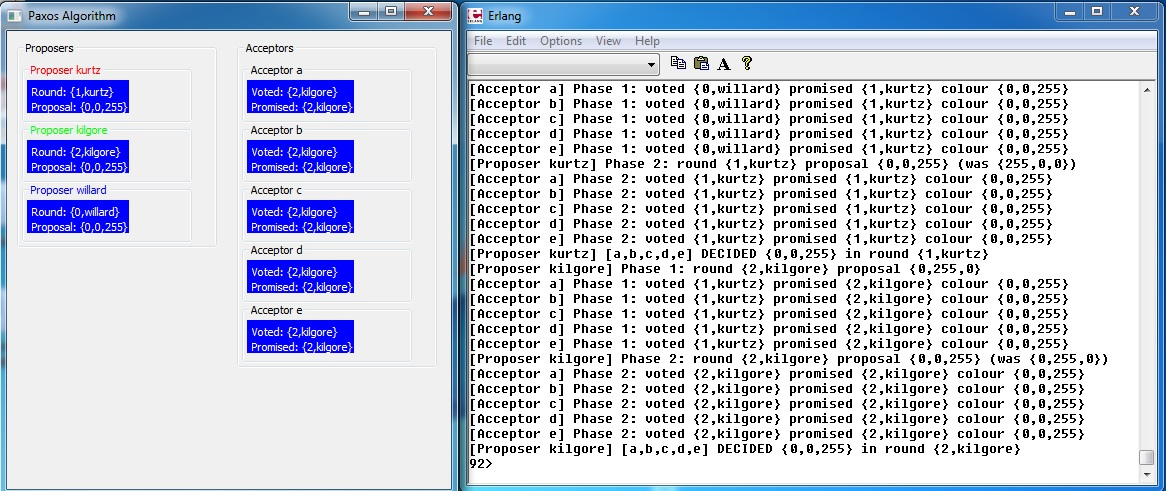
\includegraphics[width=0.95\textwidth]{./3_Experiments/images/drop_promise.jpg}
    \caption{Execution dropping promise messages \label{fig:drop_promise}}
\end{figure}
\newpage
– Experiment 2: Only drop 1/10 vote messages\newline
\begin{figure}[h!]
  \centering
    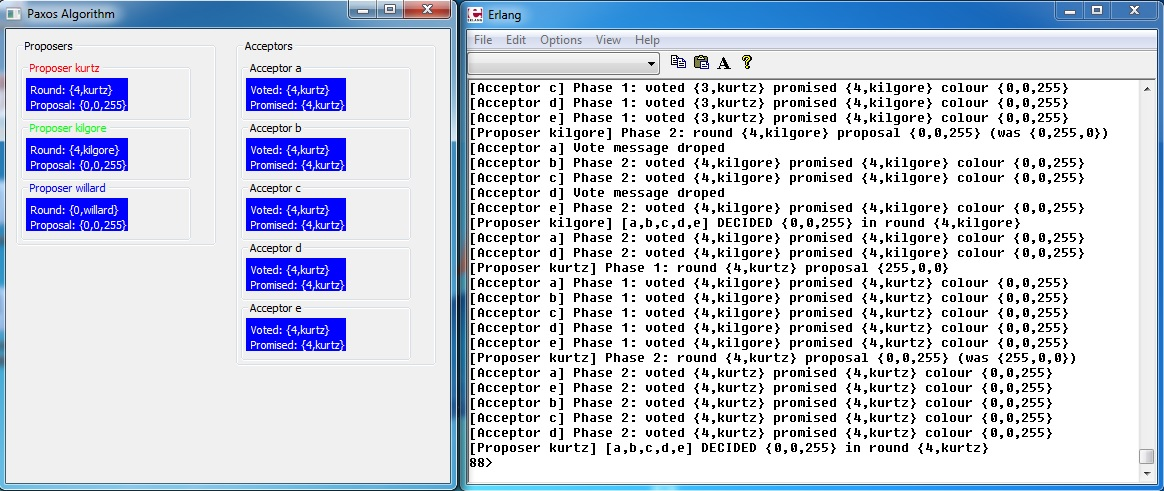
\includegraphics[width=0.95\textwidth]{./3_Experiments/images/drop_accept.jpg}
    \caption{Execution dropping accept messages\label{fig:drop_accept}}
\end{figure}

– Experiment 3: Drop both 1/10 promise and 1/10 vote messages\newline
\begin{figure}[h!]
  \centering
    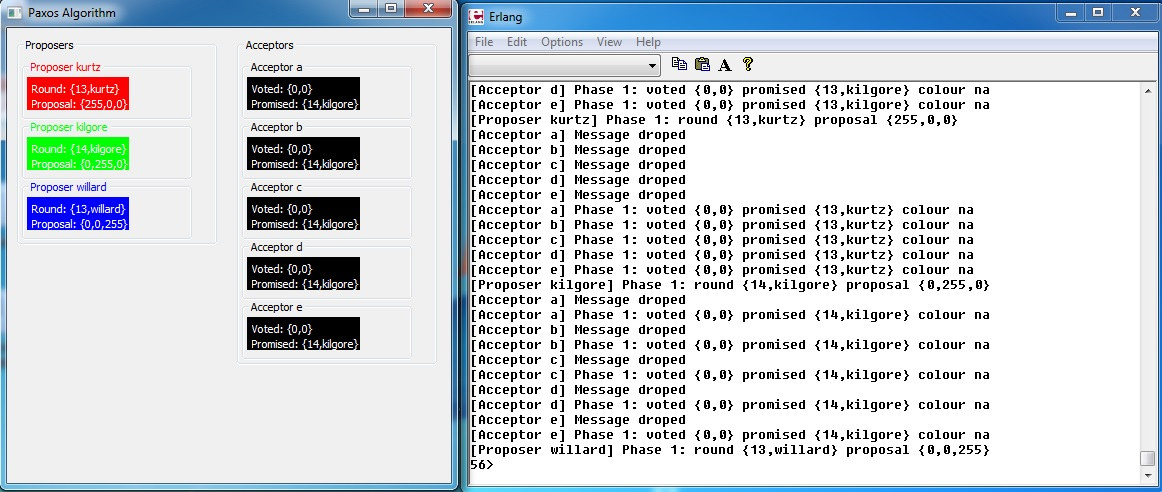
\includegraphics[width=0.95\textwidth]{./3_Experiments/images/drop_all.jpg}
    \caption{Execution dropping both promise and accept messages \label{fig:drop_all}}
\end{figure}

\begin{table}[h!]
  \centering
  \begin{tabular}{ |c | c | c | c | c |}
    \hline
                     & No drop & 1/10 Promise & 1/10 Vote & 1/10 both \\ \hline
    Number of Rounds & 1 & 1.1 & 1.13 & 2.3  \\ \hline
  \end{tabular}
  \caption{Results dropping messages in the Acceptor}
  \label{table:5}
\end{table}
As shown in Table \ref{table:5} dropping message always leads the algorithm to arrive to a consensus.
However, while promise and vote messages separately have a little and similar
effect on its execution, dropping both messages has a big effect on the algorithm
performance.

In a second set of experiments we increase the percentage of dropped messages:\newline
– drop 1/5 promise and vote messages
\begin{figure}[h!]
  \centering
    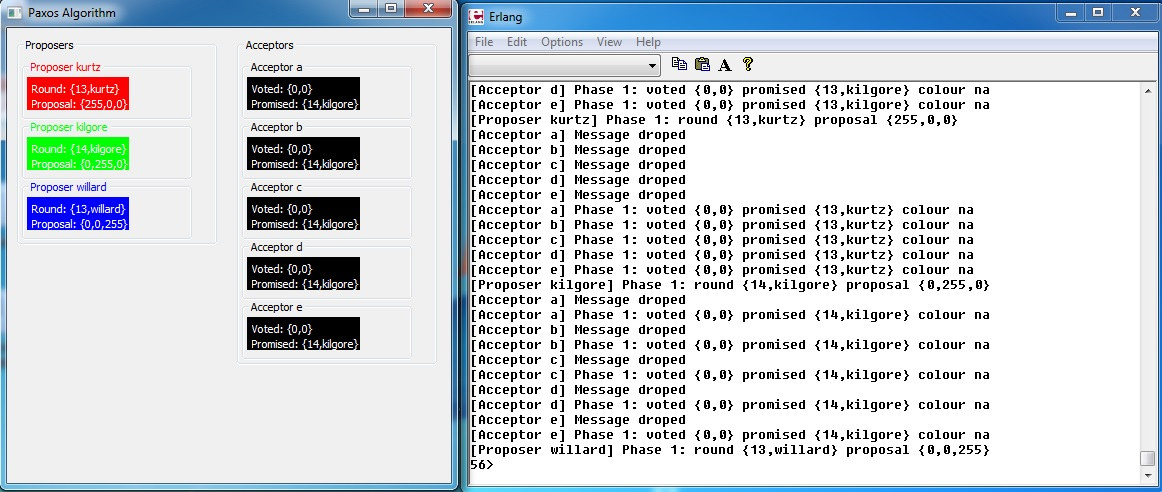
\includegraphics[width=0.95\textwidth]{./3_Experiments/images/drop_all.jpg}
    \caption{Execution dropping 1/5 messages \label{fig:drop_1}}
\end{figure}

– drop 1/2 promise and vote messages
\begin{figure}[h!]
  \centering
    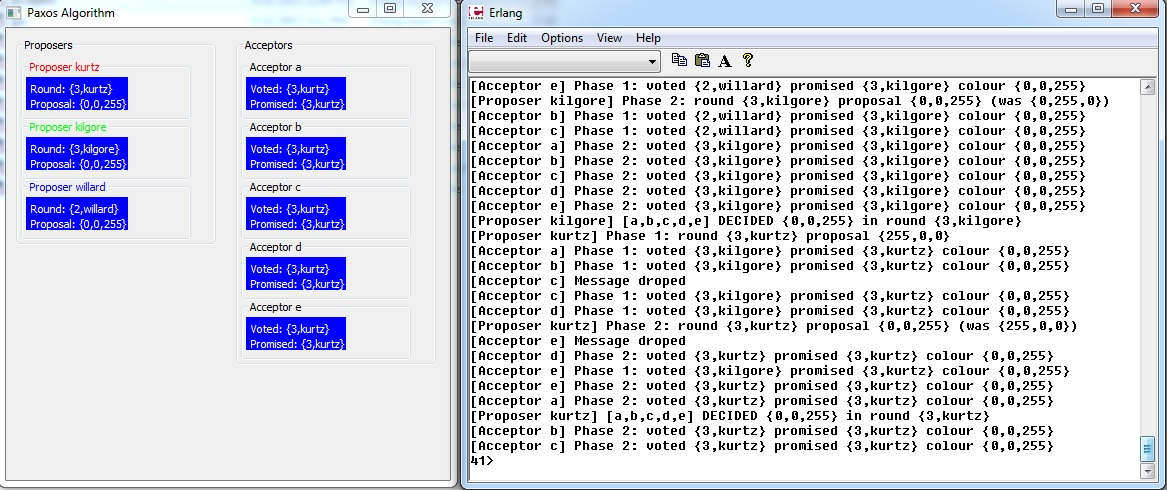
\includegraphics[width=0.95\textwidth]{./3_Experiments/images/drop_2.jpg}
    \caption{Execution dropping 1/2 messages \label{fig:drop_2}}
\end{figure}

– drop all promise and vote messages

\begin{table}[h!]
  \centering
  \begin{tabular}{ |c | c | c | c | c |}
    \hline
                     & No drop & 1/5 both & 1/2 Both & 1 both \\ \hline
    Number of Rounds & 1 & 1.23 & 6.47 & never  \\ \hline
  \end{tabular}
  \caption{Results increasing the number of dropped messages}
  \label{table:6}
\end{table}
As shown in Table \ref{table:6}, the effect of dropping a percentage of both promise and vote messages
is exponentially increasing. Moreover, it is possible that the algorithm reports
conflicting answers when a majority of accepters have voted for a proposal and
some of the vote messages are dropped. The proposer should have reach consensus 
if no messages are droped. But in the case of dropping messages, the proposer will continue.

\subsection{Increase the Number of Acceptors and Proposers}
In this experiments we increase the number of proposers and acceptors using the
basic code located under \textit{src/main}. 
Next, the experiment results are shown:\newline
• Only increase the number of acceptors 1,2,3, which means there are 3
proposers and 6,7,8 acceptors.\newline
\begin{table}[h!]
  \centering
  \begin{tabular}{ |c | c | c | c | }
    \hline
                     & [3,6] & [3,7] & [3,8] \\ \hline
    Number of Rounds & 1 & 1 & 1  \\ \hline
  \end{tabular}
  \caption{Results increasing the number of acceptors}
  \label{table:7}
\end{table}

• Only increase the number of proposers 1,2,3, which means there are
4,5,6 proposers and 5 acceptors.\newline
\begin{table}[h!]
  \centering
  \begin{tabular}{ |c | c | c | c | }
    \hline
                     & [4,5] & [5,5] & [6,5] \\ \hline
    Number of Rounds & 1.5 & 1.68 & 0  \\ \hline
  \end{tabular}
  \caption{Results increasing the number of proposers}
  \label{table:8}
\end{table}

• Increase the number of both acceptors and proposers {1,1},{2,2},{3,3}
which means there are 4 proposers 6 acceptors, 5 proposers 7 acceptors
and 6 proposers 8 acceptors.\newline
\begin{table}[h!]
  \centering
  \begin{tabular}{ |c | c | c | c| }
    \hline
                     & [4,6] & [5,7] & [6,8] \\ \hline
    Number of Rounds & 1.5 & 1.92 & 2.38  \\ \hline
  \end{tabular}
  \caption{Results increasing the number of both acceptors and proposers}
  \label{table:9}
\end{table}

As is shown in Table \ref{table:7}, Table \ref{table:8} and Table \ref{table:9}, the number
of acceptors has no effect on the number of rounds it takes for proposers 
to reach consensus. However, the number of proposers has a big effect, and
the larger the number is, the more rounds it will need to reach consensus.

\subsection{Split the PAXY Module}
The goal of this set of experiments is to run the \textit{Acceptors} and the
\textit{Proposers} on different machines. For this purpose the code saved
under the \textit{src/splitPaxy} folder have been developped. The gui.erl has been
modified to allow separated gui's for \textit{Acceptors} and \textit{Proposers} and
the paxy.erl module has been modified to start separately \textit{Acceptors} and \textit{Proposers}.

When starting Erlang, we make it network aware by providing a name: \newline
• erl -sname acceptors -setcookie 123456 \newline
• erl -sname proposers -setcookie 123456 \newline

Then, Erlang processes can communicate with each other in different machines by
using the following command: \newline
\textit{\{ACCEPTOR\_ID, acceptors@NODE\_NAME\} ! message}

\begin{figure}[h!]
  \centering
    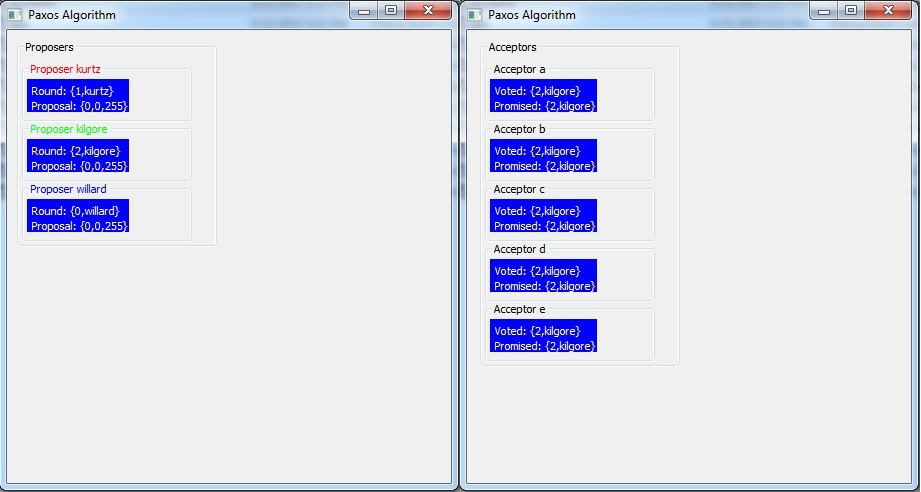
\includegraphics[width=0.95\textwidth]{./3_Experiments/images/split.jpg}
    \caption{Execution of split PAXY \label{fig:split}}
\end{figure}
Figure \ref{fig:split} shows the execution after splitting the PAXY module.

\subsection{Fault Tolerance}
For this experiment we have added the pers module to the acceptor so it can save
and restore its state. Basically we have added the pers:open(Name) and pers:read(Name) 
method calls in \textit{Acceptor} init(Name,PaneId) and the pers:store(...) every
time that the \textit{Acceptor} updates its state. The code used for these experiments
can be found under the \textit{src/faultTolerance} folder.
In order to make sure the acceptor really recovers, we do two experiments:\newline
• Not restart the acceptor after exiting\newline
\begin{figure}[h!]
  \centering
    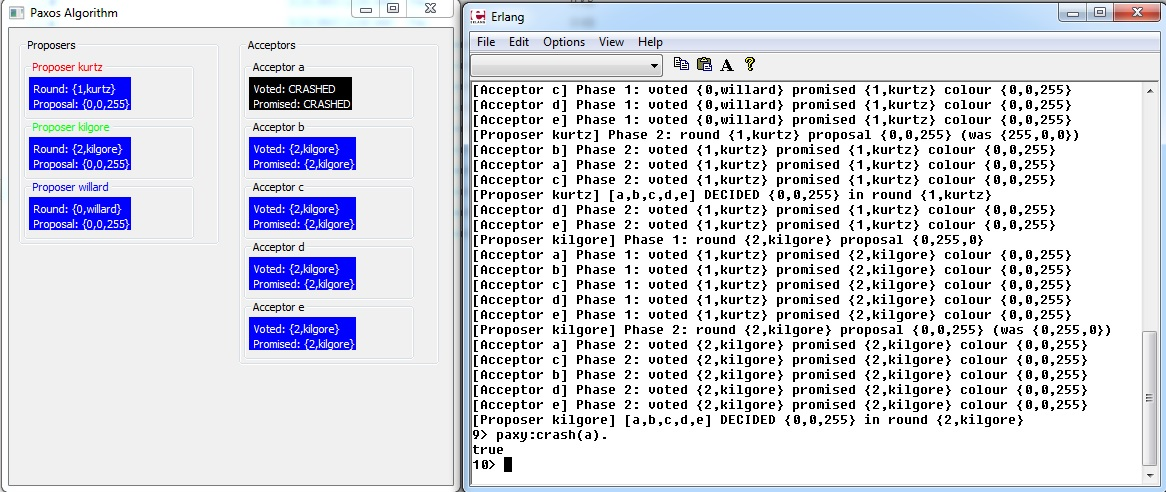
\includegraphics[width=0.95\textwidth]{./3_Experiments/images/faulttolerance1.jpg}
    \caption{Execution of fault tolerance without restart \label{fig:faulttolerance1}}
\end{figure}
• Restart the acceptor after exiting\newline
\begin{figure}[h!]
  \centering
    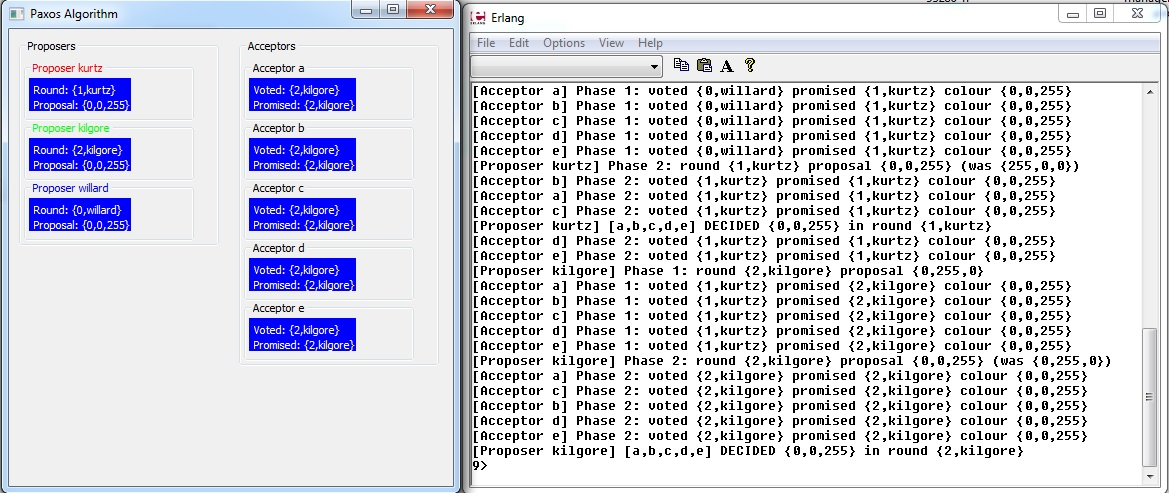
\includegraphics[width=0.95\textwidth]{./3_Experiments/images/faulttolerance2.jpg}
    \caption{Execution of fault tolerance with restart \label{fig:faulttolerance2}}
\end{figure}

A shown in Figure \ref{fig:faulttolerance1}, when \textit{Acceptor 1} is not restarted 
after exiting, it remains crashed and never recovers. However, as shown in Figure
\ref{fig:faulttolerance2} when the acceptor is restarted after exiting, it recovers
and the algorithm can reach a consensus. Therefore, we can conclude that our fault
tolerance version works well after crashing.

\subsection{Improvement Based on Sorry Message}
After receiving sorry messages from a majority of acceptors, it means the
proposer will never receive promise messages or vote messages from a majority
of acceptors. Therefore, the ballot will abort in order to get better efficiency. For
this experiments we modify the collect and vote methods in the \textit{proposer} code
adding a parameter to count the recieved sorry messages. The code can be found
under the \textit{src/sorryImprovement} folder. 
\begin{figure}[h!]
  \centering
    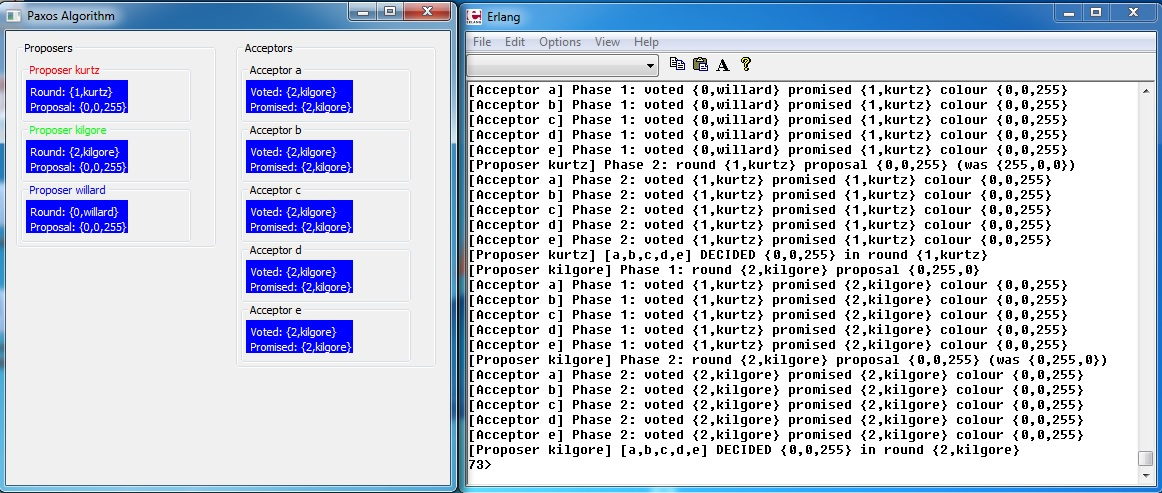
\includegraphics[width=0.95\textwidth]{./3_Experiments/images/sorryImprovement.jpg}
    \caption{Execution of fault tolerance with restart \label{fig:sorryImprovement}}
\end{figure}
\newpage
After having executed this new version we can check that the ballot is aborted earlier
and thus, it achieves the next round more efficiently. 
